\documentclass[11pt,a4paper]{article}
\usepackage[es-CL]{datetime2} 
\DTMsetdatestyle{ddmmyyyy}     
\DTMsetup{datesep=/}   
% ===================== Codificación y fuentes =====================
\usepackage[utf8]{inputenc}
\usepackage[T1]{fontenc}

% ===================== Página y utilidades ========================
\usepackage[left=2.5cm,right=2.5cm,top=2.5cm,bottom=2.5cm]{geometry}
\usepackage{array}
\usepackage{enumitem}
\usepackage{graphicx}
\usepackage{xcolor}
\usepackage{titlesec}
\usepackage{fancyhdr}
\usepackage[most]{tcolorbox}
\usepackage{hyperref}
\usepackage{booktabs}
\usepackage{amsmath}
\usepackage{caption}
\usepackage{subcaption}
\usepackage{multirow}

% ===================== Etiquetas en español (sin babel) ===========
\renewcommand{\contentsname}{Índice}
\renewcommand{\figurename}{Figura}
\renewcommand{\tablename}{Tabla}
\renewcommand{\refname}{Bibliografía}

% ===================== Escala de grises (sin color) ================
\definecolor{negro}{RGB}{0,0,0}
\definecolor{gris}{RGB}{90,90,90}
\definecolor{grisclaro}{RGB}{150,150,150}
\definecolor{fillgray}{RGB}{175,175,175}

% ===================== Hipervínculos (negro) =======================
\hypersetup{colorlinks=true, linkcolor=negro, urlcolor=negro, citecolor=negro}

% ===================== Estilo de títulos ===========================
\titleformat{\section}{\large\bfseries\color{negro}}{\thesection.}{0.5em}{}
\titleformat{\subsection}{\normalsize\bfseries\color{negro}}{\thesubsection}{0.5em}{}
\titlespacing*{\section}{0pt}{1.4em}{0.4em}
\titlespacing*{\subsection}{0pt}{1.0em}{0.3em}

% ===================== Pie de página ===============================
\pagestyle{fancy}
\fancyhf{}
\fancyfoot[L]{\footnotesize\color{gris}Magíster en Ciencia de Datos e Inteligencia Artificial}
\fancyfoot[R]{\footnotesize\color{gris}\thepage}
\renewcommand{\headrulewidth}{0pt}
\renewcommand{\footrulewidth}{0.4pt}

% ===================== Comandos del docente ========================
\newcommand{\guia}[1]{{\small\itshape\color{gris}#1}\par\vspace{0.15em}}

% Caja de información de la evaluación:
\newtcolorbox{infobox}[1][Información de la evaluación]{colback=black!3,colframe=negro,
  fonttitle=\bfseries,coltitle=white,title={#1},boxrule=0.6pt,arc=1pt,
  left=8pt,right=8pt,top=6pt,bottom=6pt,breakable}

% Caja de conexión con evaluaciones previas:
\newtcolorbox{conexionbox}[1][Conexión con evaluaciones anteriores]{colback=black!6,colframe=gris,
  fonttitle=\bfseries,coltitle=white,title={#1},boxrule=0.6pt,arc=1pt,
  left=8pt,right=8pt,top=6pt,bottom=6pt,breakable}

% Caja de resultados estadísticos:
\newtcolorbox{resultbox}[1][Resultado]{colback=black!4,colframe=grisclaro,
  fonttitle=\bfseries,coltitle=negro,title={#1},boxrule=0.5pt,arc=1pt,
  left=8pt,right=8pt,top=5pt,bottom=5pt,breakable}

% ===================== Datos del grupo ===========================
\newcommand{\proyTitulo}{Análisis Estadístico de Deserción en Educación Superior}
\newcommand{\proyIntegrantes}{
%
- Pablo Ignacio Balbontín Constenla \\
- Melany Esmeralda Reyes Leiva \\
- Ingeborg Andrea Muñoz Carnot \\
- Mario Alejandro López Pulgar%
}
\newcommand{\proyDataset}{Predict Students' Dropout and Academic Success (UCI, 2022)}
\newcommand{\proyDocente}{Jean Paul Maidana González}
\newcommand{\proyFecha}{\today}
\newcommand{\proyRepo}{\url{https://github.com/dark452/mcdi501-grupo1}}

\setlength{\parindent}{0pt}
\setlength{\parskip}{0.4em}

\begin{document}
\pagenumbering{gobble}

% ================================================================
% PORTADA
% ================================================================
\thispagestyle{empty}
\begin{center}
\vspace*{1.0cm}

\includegraphics[height=4.4cm]{logo_unab.png}\\[1.3cm]

{\footnotesize\color{gris}\MakeUppercase{Magíster en Ciencia de Datos e Inteligencia Artificial}}\\[0.15cm]
{\footnotesize\color{grisclaro}MCDI501: Estadística Computacional para la Toma de Decisiones}\\[2.0cm]

{\Large\bfseries\color{negro} Evaluación Sumativa 1}\\[0.45cm]
{\large\color{negro} Análisis Exploratorio e Inferencial}\\[1.0cm]

{\small\itshape\color{gris} Informe técnico grupal \textperiodcentered\ 20\,\%}
\end{center}

\vspace{1.6cm}

\begin{flushleft}
\setlength{\extrarowheight}{5pt}
\begin{tabular}{@{}>{\bfseries\color{negro}}l l@{}}
Título del proyecto: & \proyTitulo \\
Integrantes:         & \begin{tabular}[t]{@{}l@{}} \proyIntegrantes \end{tabular} \\
Dataset:             & \proyDataset \\
Docente:             & \proyDocente \\
Fecha:               & \proyFecha \\
Repositorio GitHub:  & \proyRepo \\
\end{tabular}
\end{flushleft}

\clearpage
\pagenumbering{arabic}

% ================================================================
% CAJA DE INFO
% ================================================================
\begin{infobox}
\textbf{Fase del proyecto:} Fase 2: Análisis Exploratorio e Inferencial\\
\textbf{Modalidad:} Grupal (3--4 integrantes)\qquad\textbf{Ponderación:} 20\,\% de la nota final\\
\textbf{Entregables:} Informe PDF (máx.\ 8 págs., sin anexos)\ \textperiodcentered\ Notebook \texttt{.ipynb}\ \textperiodcentered\ Repositorio GitHub\\
\textbf{Resultado de aprendizaje (RA1):} aplicar probabilidad e inferencia estadística en problemas de decisión bajo incertidumbre.\\
\textbf{Indicadores:} ID1.2, ID1.3, ID1.4.
\end{infobox}

\vspace{0.5em}
\tableofcontents
\newpage

% ================================================================
% SECCIÓN 1
% ================================================================
\section{Preparación y carga de datos}

\subsection{Descripción del dataset}

El dataset \textit{Predict Students' Dropout and Academic Success} \cite{realinho2022} contiene registros de 4,424 estudiantes de una institución de educación superior portuguesa. Reúne información recopilada al momento de la matrícula (atributos socioeconómicos y demográficos), el desempeño académico del primero y segundo semestre, y variables de contexto macroeconómico. La variable objetivo (\texttt{Target}) clasifica a cada estudiante en una de tres categorías: \textit{Dropout}, \textit{Enrolled} y \textit{Graduate}.

El archivo fuente utiliza punto y coma como delimitador (\texttt{sep=';'}). Se realizó limpieza de nombres de columnas eliminando espacios y caracteres de tabulación residuales, sin requerir transformaciones adicionales.

\subsection{Clasificación de variables}

El dataset contiene 37 variables que se clasifican en cuatro grupos:

\begin{itemize}[noitemsep]
    \item \textbf{Numéricas continuas (7):} Nota de calificación previa, Nota de admisión, Nota 1\textsuperscript{er} semestre, Nota 2\textsuperscript{do} semestre, Tasa de desempleo, Tasa de inflación, PIB.
    \item \textbf{Numéricas discretas (6):} Edad al matricularse, unidades curriculares inscritas y aprobadas por semestre, orden de postulación.
    \item \textbf{Categóricas nominales (9):} Estado civil, modo de postulación, curso, nacionalidad, calificación y ocupación de los padres.
    \item \textbf{Categóricas binarias (8):} Asistencia diurna/vespertina, desplazado, necesidades educativas especiales, deudor, matrícula al día, género, becado, estudiante internacional.
    \item \textbf{Variable objetivo (1):} \texttt{Target},  resultado académico del estudiante.
\end{itemize}

\subsection{Reporte de calidad de los datos}

\begin{table}[h!]
\centering
\begin{tabular}{lc}
\toprule
\textbf{Dimensión de calidad} & \textbf{Resultado} \\
\midrule
Registros totales              & 4,424 \\
Variables totales              & 37 \\
Valores faltantes              & 0 (0.0\,\%) \\
Registros duplicados           & 0 \\
Variables con rango anómalo    & 0 \\
Nombre de columnas corregidos  & 1 (tab residual en \texttt{Daytime/evening attendance}) \\
\bottomrule
\end{tabular}
\caption{Reporte inicial de calidad del dataset}
\end{table}

El dataset presenta una calidad de datos excepcional: no requiere imputación de valores faltantes ni eliminación de filas. Los rangos de todas las variables se encuentran dentro de los valores esperados para el dominio (notas de admisión en [95, 190] según el sistema ENES portugués, notas semestrales en [0, 20]). Esta condición permite proceder directamente al análisis exploratorio sin preprocesamiento adicional.

% ================================================================
% SECCIÓN 2
% ================================================================
\newpage
\section{Análisis exploratorio de datos}


\subsection{Distribución de la variable objetivo}

La variable \texttt{Target} presenta la distribución mostrada en la Figura~\ref{fig:target}: el 49.9\,\% de los estudiantes se gradúa (n=2,209), el 32.1\,\% abandona (n=1,421) y el 17.9\,\% permanece matriculado (n=794). El desequilibrio de clases debe considerarse al desarrollar modelos predictivos en fases posteriores.

\begin{figure}[h!]
\centering
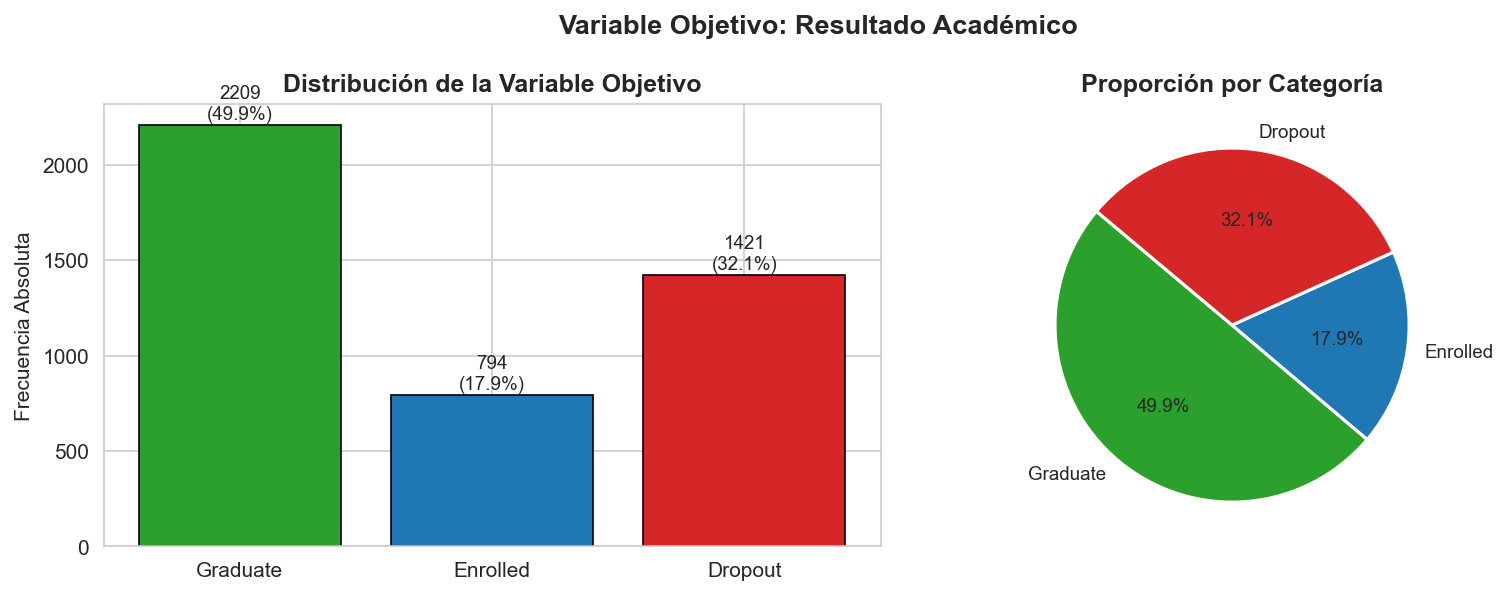
\includegraphics[width=0.82\textwidth]{fig1_distribucion_target.png}
\caption{Distribución de frecuencias de la variable objetivo \texttt{Target}.}
\label{fig:target}
\end{figure}

\subsection{Estadística descriptiva de variables numéricas}

La Tabla~\ref{tab:desc} presenta las medidas de tendencia central, dispersión y forma para las ocho variables numéricas principales.

\begin{table}[h!]
\centering
\small
\begin{tabular}{lrrrrrrrrl}
\toprule
\textbf{Variable} & \textbf{Media} & \textbf{Moda} & \textbf{DE} & \textbf{CV(\%)} & \textbf{Mín} & \textbf{Mediana} & \textbf{Máx} & \textbf{Asim.}  &\textbf{Curtosis}\\
\midrule
Nota Cal. Anterior   & 132.61 & 133.10 & 13.19 & 9.9  &  95.0 & 133.1 & 190.0 & $+$0.31  &0.968\\
Nota de Admisión     & 126.98 & 130.00 & 14.48 & 11.4 &  95.0 & 126.1 & 190.0 & $+$0.53  &0.663\\
Edad Matrícula       &  23.27 & 18.00 & 7.59 & 32.6 &  17.0 &  20.0 &  70.0 & $+$2.05  &4.127\\
Nota 1\textsuperscript{er} Sem.  &  10.64 & 0.00 & 4.84 & 45.5 &   0.0 &  12.3 &  18.9 & $-$1.56  &0.908\\
Nota 2\textsuperscript{do} Sem.  &  10.23 & 0.00 & 5.21 & 50.9 &   0.0 &  12.2 &  18.6 & $-$1.35  &0.067\\
Tasa Desempleo       &  11.57 & 7.60 & 2.66 & 23.0 &   7.6 &  11.1 &  16.2 & $+$0.21  &-0.996\\
Tasa Inflación       &   1.23 & 1.40 & 1.38 & 112.3 & $-$0.8 &  1.4 &   3.7 & $+$0.25  &-1.039\\
PIB                  &   0.00 & 0.32 & 2.27 & --- & $-$4.1 &   0.3 &   3.5 & $-$0.37  &-1.002\\
\bottomrule
\end{tabular}
\caption{Estadísticos descriptivos de variables numéricas (n = 4,424)}
\label{tab:desc}
\end{table}

\begin{figure}[h!]
\centering
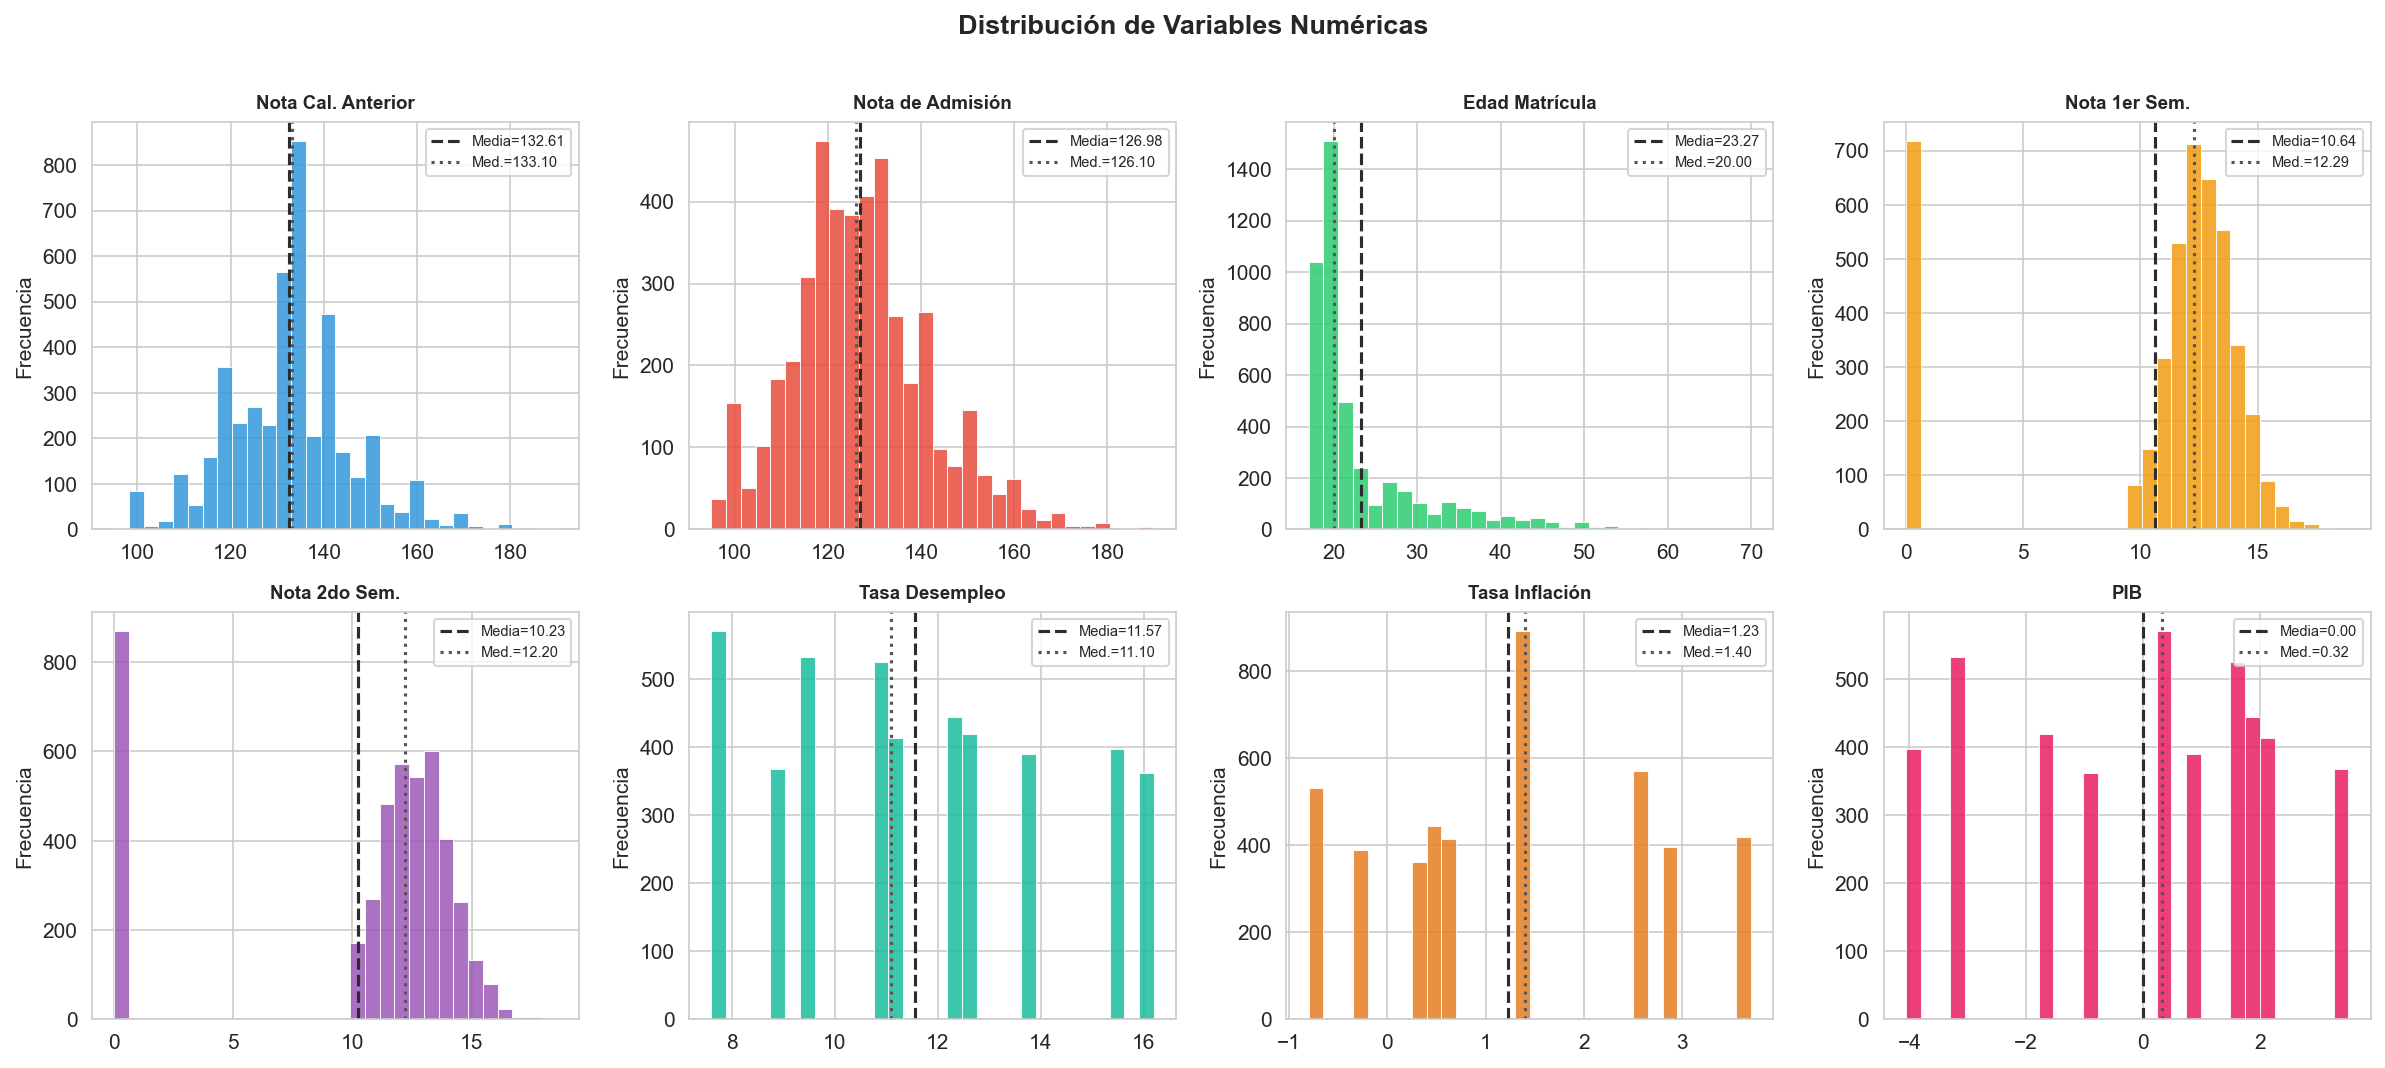
\includegraphics[width=\textwidth]{fig2_histogramas.png}
\caption{Histogramas de las variables numéricas con líneas de media (---) y mediana (\textperiodcentered\textperiodcentered\textperiodcentered).}
\label{fig:hist}
\end{figure}

Los histogramas (Figura~\ref{fig:hist}) revelan que las notas académicas semestrales presentan distribuciones bimodales con un pico pronunciado en cero, correspondiente a estudiantes que abandonaron sin completar evaluaciones. La edad al matricularse muestra la asimetría positiva más marcada (coeficiente = 2.05), con mayoría de estudiantes jóvenes (moda $\approx$ 18 años) y cola hacia edades adultas.

\subsection{Variables categóricas: frecuencias y representación gráfica}

\begin{figure}[h!]
\centering
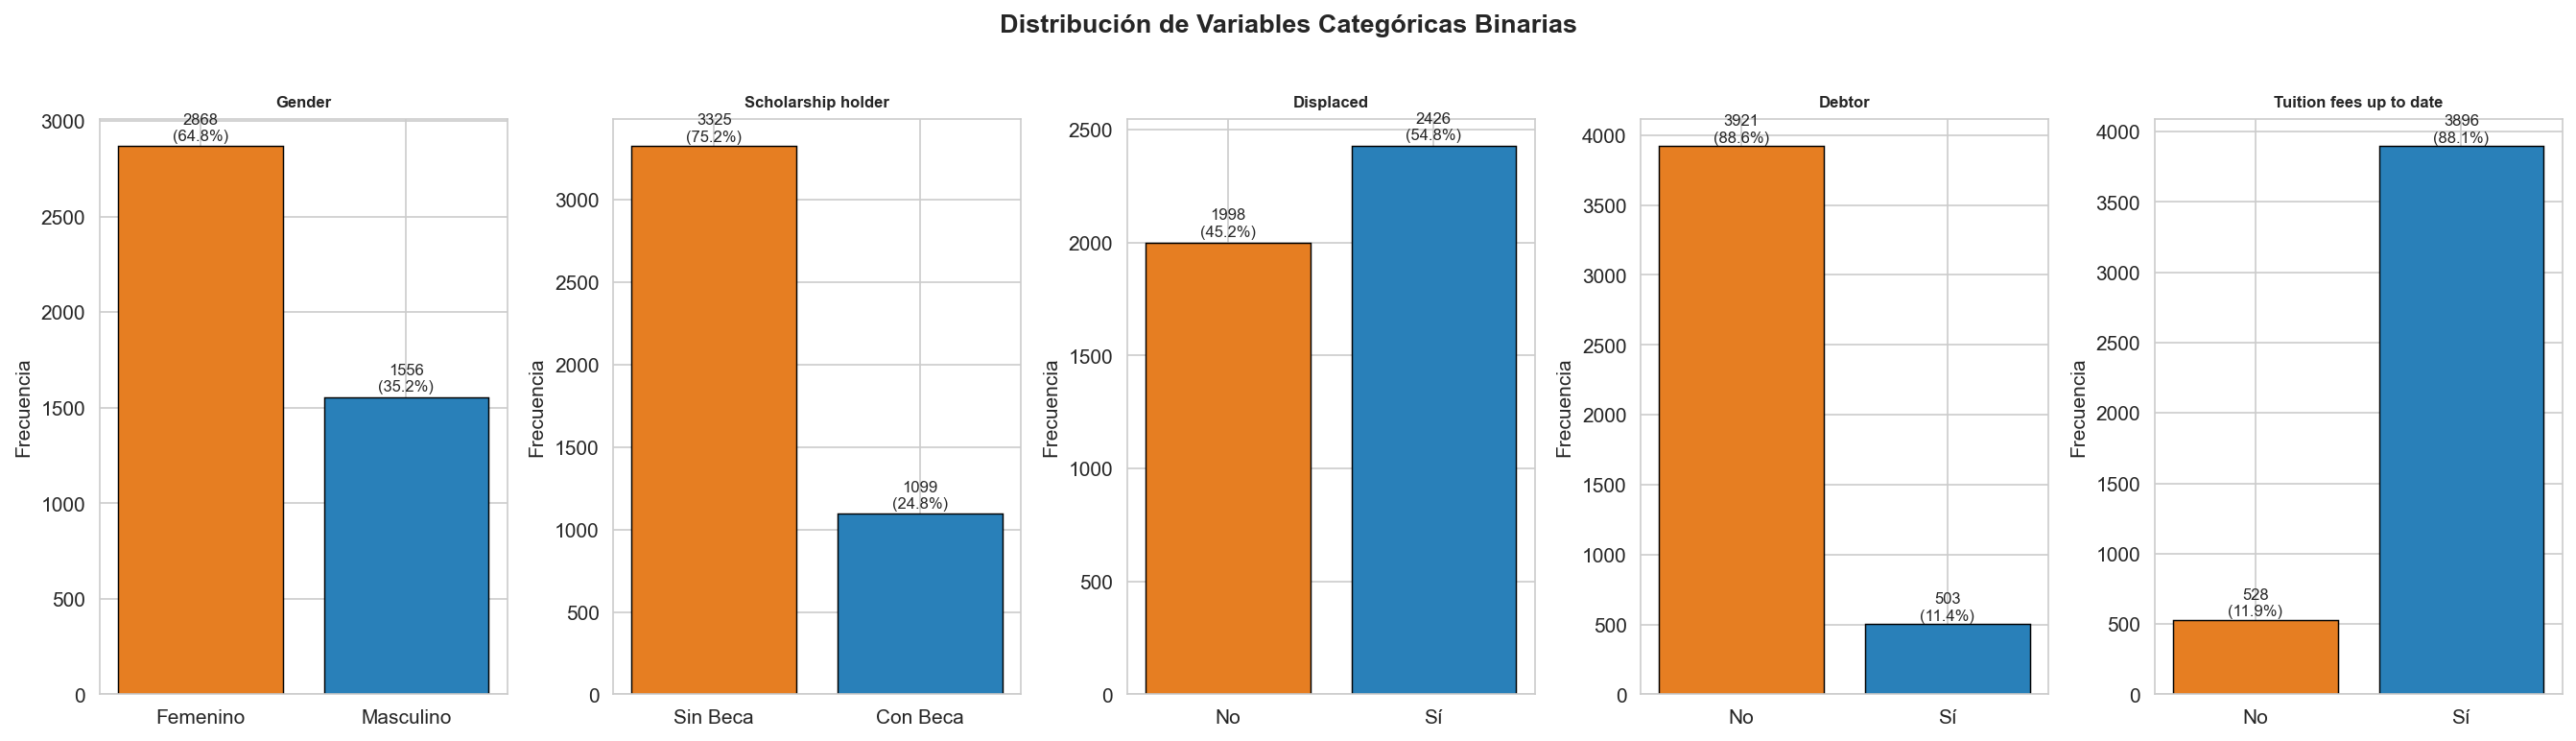
\includegraphics[width=\textwidth]{fig5_categoricas.png}
\caption{Distribución de variables categóricas binarias: frecuencia absoluta y porcentaje.}
\label{fig:cat}
\end{figure}

La muestra es predominantemente femenina (64.8\,\%, n=2,868). El 75.2\,\% de los estudiantes no cuenta con beca. El 88.1\,\% mantiene la matrícula al día y solo el 11.4\,\% registra deuda con la institución.

\subsection{Análisis bivariado}

\begin{figure}[h!]
\centering
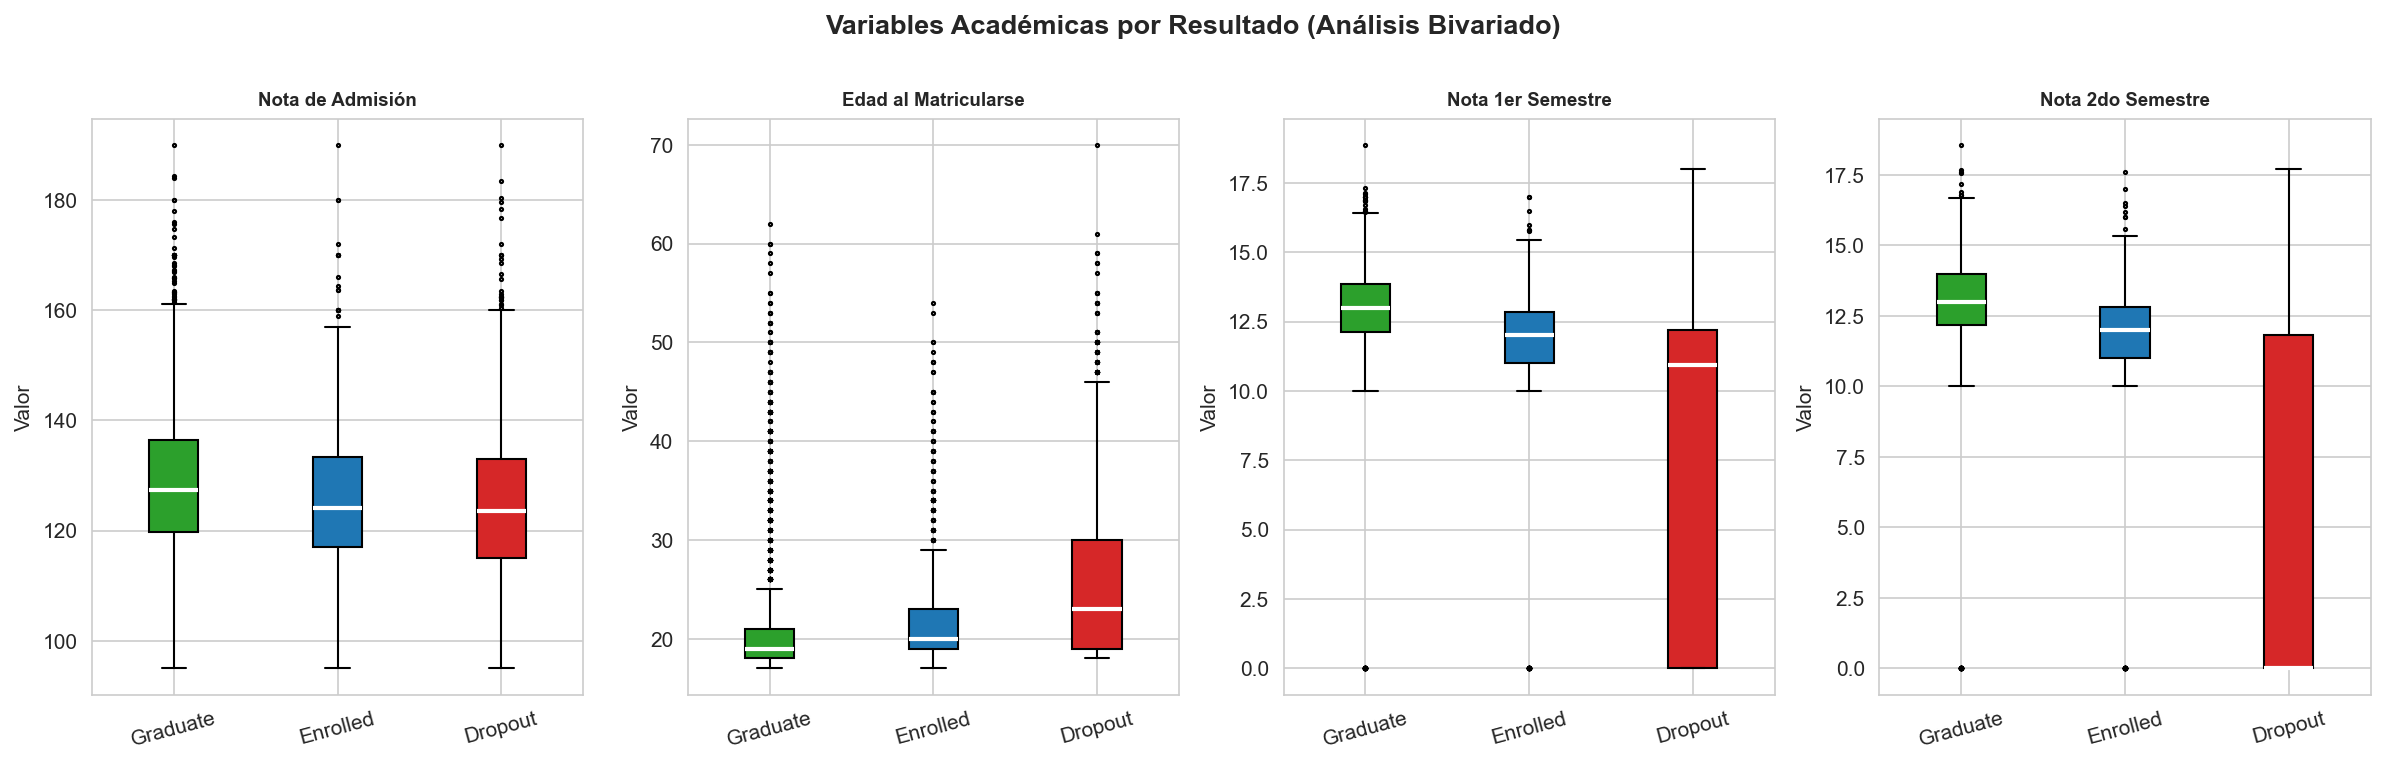
\includegraphics[width=\textwidth]{fig3_boxplots_target.png}
\caption{Boxplots de variables académicas clave según resultado (\textit{Graduate}, \textit{Enrolled}, \textit{Dropout}).}
\label{fig:boxplots}
\end{figure}

Los boxplots (Figura~\ref{fig:boxplots}) evidencian diferencias sistemáticas entre grupos. Las notas del 1\textsuperscript{er} y 2\textsuperscript{do} semestre separan con claridad a los graduados de los desertores: los primeros obtienen medianas de $\approx$12--13 puntos, mientras los desertores concentran valores cercanos a cero. La edad al matricularse muestra una tendencia inversa: los desertores son en promedio $\approx$4 años mayores que los graduados.

\begin{figure}[h!]
\centering
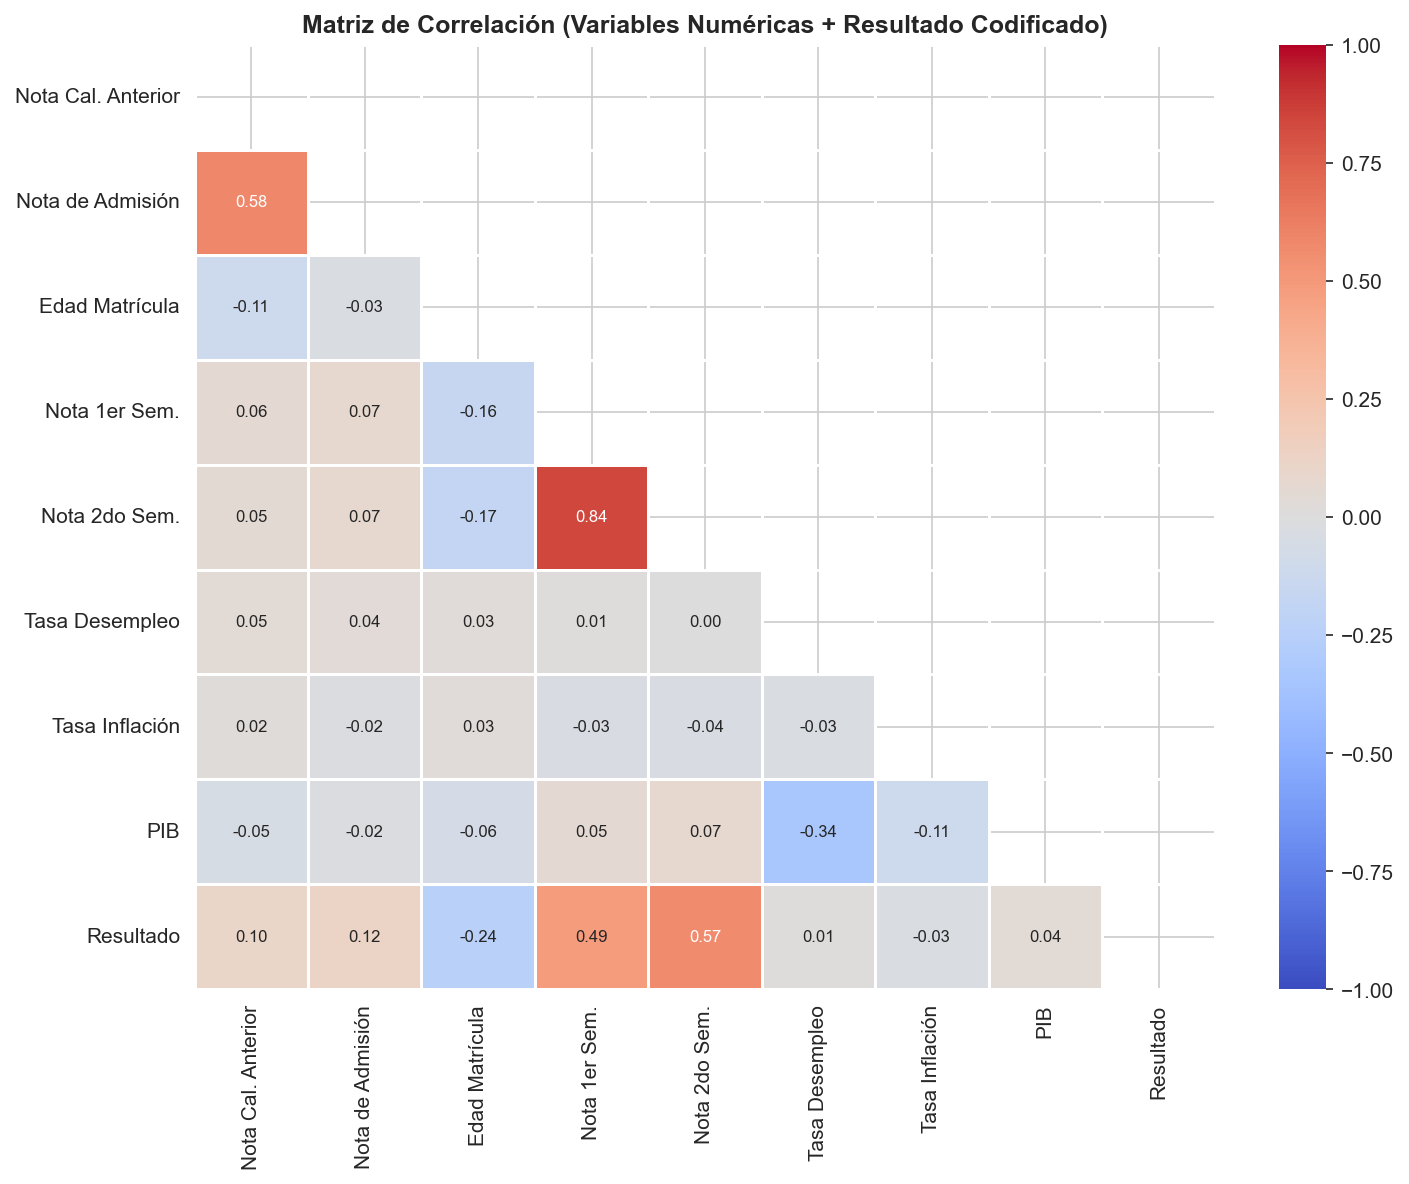
\includegraphics[width=0.80\textwidth]{fig4_correlacion.png}
\caption{Matriz de correlación de Pearson entre variables numéricas y resultado codificado.}
\label{fig:corr}
\end{figure}

La matriz de correlación (Figura~\ref{fig:corr}) confirma que la nota del 2\textsuperscript{do} semestre presenta la correlación más alta con el resultado (r=0.57), seguida por la nota del 1\textsuperscript{er} semestre (r=0.49). La edad tiene correlación negativa débil (r=$-$0.24). Las variables macroeconómicas exhiben correlaciones marginales ($|r|<0.05$), salvo el PIB (r=0.044), confirmando que el resultado depende predominantemente de factores académicos individuales.

% ================================================================
% SECCIÓN 3
% ================================================================
\section{Estimación de parámetros}


\subsection{Método y justificación}

Se emplean intervalos de confianza basados en la distribución $t$ de Student para estimación de medias poblacionales:

\[
\bar{X} \pm t_{\alpha/2,\, n-1} \cdot \frac{s}{\sqrt{n}}
\]

Este método es apropiado cuando la varianza poblacional es desconocida, independientemente del tamaño muestral. Para $n=4{,}424$, el cuantil $t_{0.025,\,4423} \approx 1.9605$ converge al valor normal estándar, pero se mantiene la fórmula exacta por rigor metodológico.

\subsection{Resultados}

\begin{table}[h!]
\centering
\begin{tabular}{lrrrr}
\toprule
\textbf{Variable} & \textbf{Media} & \textbf{DE} & \textbf{IC 95\,\% Inf.} & \textbf{IC 95\,\% Sup.} \\
\midrule
Nota de Admisión          & 126.978 & 14.482 & 126.551 & 127.405 \\
Edad al Matricularse      &  23.265 &  7.588 &  23.042 &  23.489 \\
Nota 1\textsuperscript{er} Semestre    &  10.641 &  4.844 &  10.498 &  10.784 \\
PIB                       &   0.002 &  2.270 &  $-$0.065 &   0.069 \\
\bottomrule
\end{tabular}
\label{tab:ci}
\caption{Estimaciones puntuales e intervalos de confianza al 95\,\% (n = 4,424)}
\end{table}

\begin{figure}[h!]
\centering
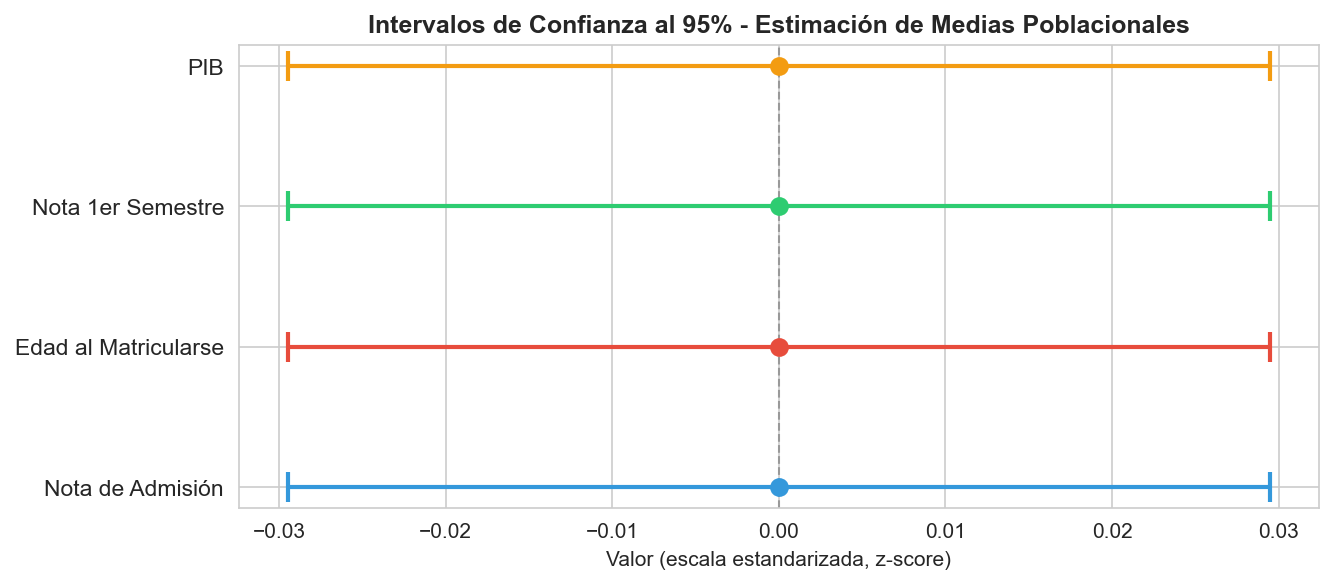
\includegraphics[width=0.75\textwidth]{fig6_intervalos_confianza.png}
\caption{Forest plot de intervalos de confianza al 95\,\% (escala estandarizada).}
\label{fig:ci}
\end{figure}

\subsection{Interpretación y limitaciones}

\textbf{Nota de Admisión} [126.55, 127.41]: El IC estrecho ($\pm$0.43 puntos) refleja la alta precisión derivada del tamaño muestral. Se estima que la nota promedio de ingreso institucional ronda los 127 puntos sobre 190 ($\approx$66.8\,\% de la escala).

\textbf{Edad al matricularse} [23.04, 23.49]: La media estimada de $\approx$23.3 años confirma una población predominantemente joven, aunque la elevada dispersión ($s=7.6$ años) indica heterogeneidad etaria relevante que la media sola no captura.

\textbf{Nota 1\textsuperscript{er} Semestre} [10.50, 10.78]: La media de 10.64 sobre 20 es inferior a la esperada para una población universitaria seleccionada. Esto se explica por la presencia de desertores con calificación cero, lo que deprime la media global.

\textbf{PIB} [$-$0.065, 0.069]: El IC incluye el cero, indicando que el crecimiento económico medio durante el período cubierto no difiere significativamente de cero. Esto refleja la volatilidad del contexto económico portugués post-crisis 2008.

\textbf{Nota metodológica sobre variables macroeconómicas:} El PIB, la tasa de
desempleo y la inflación no constituyen mediciones independientes por
estudiante, sino valores compartidos por cohortes de matrícula del mismo
período. En consecuencia, el error estándar reportado en la Tabla 3 subestima
la variabilidad real del parámetro macroeconómico, ya que trata a $n=4{,}424$
observaciones como independientes cuando el número efectivo de períodos
distintos en el dataset es sustancialmente menor. El intervalo debe
interpretarse como una descripción del promedio observado en la muestra,
no como una estimación inferencial estricta del parámetro poblacional.

\textbf{Limitaciones:} 
\begin{enumerate}
    \item Los IC asumen muestreo aleatorio, si el dataset tiene sesgo institucional, las estimaciones pueden no generalizarse a otras instituciones. 
    \item Para variables asimétricas (como edad), el IC para la mediana o percentiles sería más informativo que el IC para la media.
\end{enumerate}



% ================================================================
% SECCIÓN 4
% ================================================================
\section{Pruebas de hipótesis}


\subsection{Prueba 1: Diferencia en nota de admisión entre desertores y graduados}

\textbf{Prueba:} $t$ de Welch (dos muestras independientes)

\begin{itemize}[noitemsep]
    \item $H_0: \mu_{\text{Dropout}} = \mu_{\text{Graduate}}$ (la nota media de admisión es igual en ambos grupos)
    \item $H_1: \mu_{\text{Dropout}} \neq \mu_{\text{Graduate}}$ (existe diferencia significativa entre grupos)
    \item Nivel de significancia: $\alpha = 0.05$ (Es el estándar en ciencias sociales y medicina)
\end{itemize}

\textbf{Verificación de supuestos:}
\begin{itemize}[noitemsep]
    \item \textit{Normalidad:} Prueba de Shapiro-Wilk sobre submuestra de 50 observaciones por grupo. Dropout: $W=0.977$, $p=0.423$ (no se rechaza normalidad). Graduate: $W=0.938$, $p=0.011$ (se rechaza al 5\,\%). Para $n>1{,}000$, el Teorema Central del Límite garantiza normalidad asintótica de las medias, por lo que la prueba es válida.
    \item \textit{Homogeneidad de varianzas:} Prueba de Levene: $F=10.63$, $p=0.0011$. Se rechazan varianzas iguales → se aplica corrección de Welch.
\end{itemize}

\begin{resultbox}[Resultado - Prueba 1]
\begin{tabular}{ll}
Grupo Dropout  & $n=1{,}421$, $\bar{X}=124.96$, $s=15.13$ \\
Grupo Graduate & $n=2{,}209$, $\bar{X}=128.79$, $s=14.07$ \\
Diferencia de medias & $\Delta\bar{X} = 3.83$ puntos \\
Estadístico $t$ de Welch & $t = -7.66$ \\
Valor $p$ (bilateral)    & $p < 0.001$ \\
Decisión & \textbf{Rechazar $H_0$} ($\alpha = 0.05$) \\
\end{tabular}
\end{resultbox}

\begin{figure}[h!]
\centering
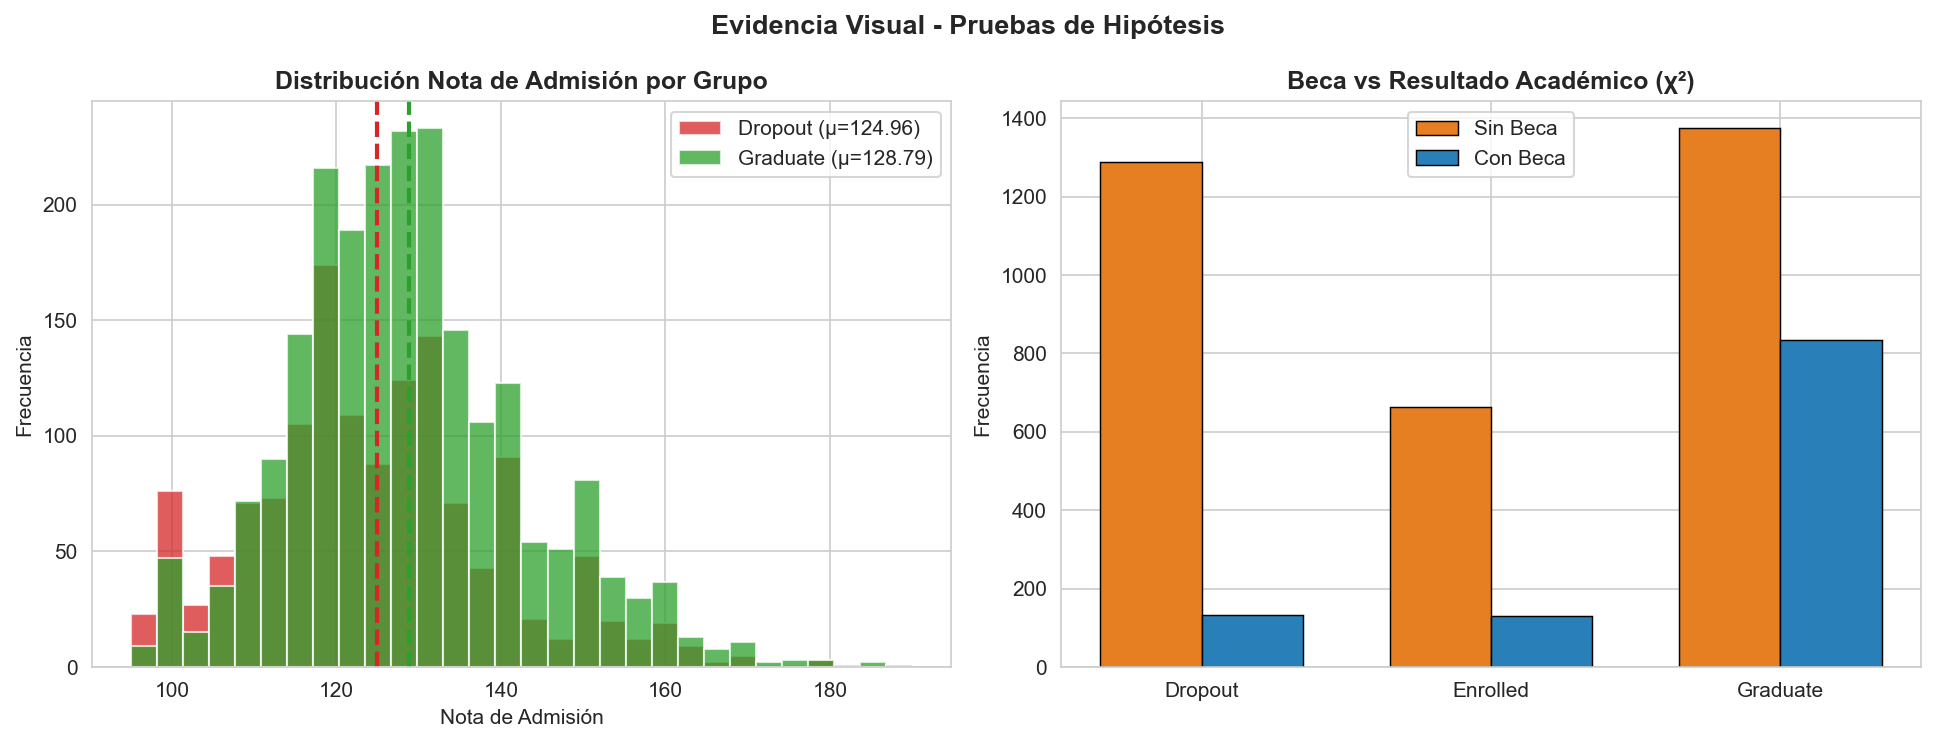
\includegraphics[width=\textwidth]{fig7_hipotesis.png}
\caption{Izquierda: distribuciones de nota de admisión por grupo (Prueba 1). Derecha: frecuencia por resultado según condición de beca (Prueba 2).}
\label{fig:tests}
\end{figure}

\textbf{Implicancias prácticas:} Con $p<0.001$ se rechaza $H_0$: los graduados presentan notas de admisión significativamente más altas. No obstante, el tamaño del efecto es pequeño (d de Cohen $\approx 0.27$), lo que indica que la nota de admisión tiene un poder discriminante limitado a nivel individual. Las notas semestrales constituyen predictores más potentes y oportunos para intervenciones de retención.

\subsection{Prueba 2: Asociación entre beca y resultado académico}

\textbf{Prueba:} Chi-cuadrado de independencia ($\chi^2$)

\begin{itemize}[noitemsep]
    \item $H_0$: La condición de becado y el resultado académico son independientes
    \item $H_1$: Existe asociación significativa entre becado y resultado
    \item Nivel de significancia: $\alpha = 0.05$
\end{itemize}

\textbf{Verificación de supuestos:} Tabla de contingencia $2 \times 3$. Frecuencia esperada mínima = 197.24 $> 5$, supuesto cumplido.

\begin{table}[h!]
\centering
\begin{tabular}{lrrr|r}
\toprule
 & \textbf{Dropout} & \textbf{Enrolled} & \textbf{Graduate} & \textbf{Total} \\
\midrule
Sin Beca (n=3,325) & 1,287 (38.7\,\%) & 664 (20.0\,\%) & 1,374 (41.3\,\%) & 3,325 \\
Con Beca (n=1,099) &   134 (12.2\,\%) & 130 (11.8\,\%) &   835 (76.0\,\%) & 1,099 \\
\bottomrule
\end{tabular}
\label{tab:chi2}
\caption{Tabla de contingencia - condición de beca × resultado académico}
\end{table}

\begin{resultbox}[Resultado - Prueba 2]
\begin{tabular}{ll}
Estadístico $\chi^2$   & $\chi^2 = 409.94$ \\
Grados de libertad     & $gl = 2$ \\
Valor $p$              & $p < 0.001$ \\
Cramér's $V$           & $V = 0.30$ (efecto moderado) \\
Decisión               & \textbf{Rechazar $H_0$} ($\alpha = 0.05$) \\
\end{tabular}
\end{resultbox}

\textbf{Implicancias prácticas:} La evidencia estadística confirma que la condición de becado está fuertemente asociada al resultado. Los becados se gradúan en el 76.0\,\% de los casos versus el 41.3\,\% de los no becados; la tasa de abandono de los no becados (38.7\,\%) triplica la de los becados (12.2\,\%). Un Cramér's $V=0.30$ indica que el efecto es moderado y prácticamente relevante: ampliar la cobertura de becas podría constituir una intervención de retención costo-efectiva. Sin embargo, debe considerarse el posible sesgo de selección: estudiantes más motivados también son más propensos a obtener becas.

% ================================================================
% SECCIÓN 5
% ================================================================

\section{Informe de avance del proyecto}

\subsection{Introducción al problema}

La deserción universitaria genera consecuencias en múltiples dimensiones:
pérdida de capital humano para el estudiante, reducción de ingresos e
indicadores de alerta para la institución, y suboptimización del gasto
público para el sistema educativo. Portugal presenta tasas de abandono
superiores a la media de la OCDE, lo que otorga especial relevancia al
dataset analizado. El objetivo del proyecto es identificar los factores
estadísticamente asociados al abandono y construir el marco analítico para
el modelamiento predictivo en las Sumativas~2 y~3.

\subsection{Descripción de métodos aplicados}

Se aplicaron en secuencia: auditoría de calidad de datos (sección~1.3),
estadística descriptiva univariada y bivariada (sección~2), estimación
puntual e intervalos de confianza al 95\,\% mediante distribución
$t$ de Student (sección~3), y pruebas de hipótesis  ($t$ de Welch y
$\chi^2$ de independencia) con verificación de supuestos y cálculo de tamaño del efecto (sección~4).


\subsection{Resumen de resultados}

Los resultados convergen en tres hallazgos centrales:

\begin{enumerate}
    \item \textbf{El rendimiento semestral es el predictor dominante.} Las notas del 1\textsuperscript{er} y 2\textsuperscript{do} semestre presentan las correlaciones más altas con el resultado (r=0.49 y r=0.57 respectivamente). Los desertores obtienen notas cercanas a cero en sus evaluaciones, lo que refleja que muchos abandonan sin completar el período académico.
    \item \textbf{La edad de matrícula es un factor de riesgo relevante.} Los desertores tienen en promedio 4.3 años más al matricularse que 
    los graduados (26.1 vs.\ 21.8 años), diferencia consistente con los patrones observados en los boxplots (Figura 4) y con la correlación negativa moderada identificada en la matriz de correlación 
(r\,=\,$-$0.24). Los estudiantes adultos enfrentan mayores barreras de permanencia, probablemente por carga laboral y responsabilidades familiares.
    \item \textbf{La beca es el factor externo con mayor asociación práctica.} La tasa de graduación entre becados (76.0\,\%) más que duplica la de no becados (41.3\,\%), con un efecto de tamaño moderado (Cramér's $V=0.30$).
\end{enumerate}


\subsection{Próximos pasos}

\begin{enumerate}[noitemsep]
    \item \textbf{Ingeniería de variables (S2):} Construir métricas de eficiencia académica (tasa de aprobación = unidades aprobadas / inscritas) que capturen el rendimiento relativo. Codificar variables nominales politómicas mediante técnicas apropiadas (target encoding, one-hot encoding).
    \item \textbf{Procedimientos de simulación y remuestreo (S2)}: Implementar procedimientos de simulación y remuestreo (Monte Carlo, bootstrap o jackknife)
    \item \textbf{Modelamiento predictivo (S2-S3):} Desarrollar modelos de clasificación multiclase: regresión logística multinomial (baseline), árbol de decisión, Random Forest y gradient boosting. Evaluar con métricas adecuadas para datos desbalanceados (F1-macro, AUC-ROC).
    \item \textbf{Balanceo de clases:} Implementar SMOTE o ajuste de pesos de clase dada la distribución desigual de \textit{Enrolled} (17.9\,\%).
    \item \textbf{Validación:} Protocolo de evaluación con $k$-fold cross-validation ($k=5$) para estimar desempeño generalizable.
%    \item \textbf{Análisis de subgrupos:} Estratificar análisis por programa académico (\texttt{Course}) para identificar cursos con mayor riesgo de abandono y orientar intervenciones específicas.
\end{enumerate}

% ================================================================
% SECCIÓN 6
% ================================================================
\section{Notebook y repositorio GitHub}

%\guia{Notebook reproducible, documentado y coherente con el informe; repositorio GitHub enlazado.}

El notebook \texttt{\href{https://github.com/dark452/mcdi501-grupo1/blob/main/notebooks/F2.ipynb}{notebooks/F2.ipynb}} está disponible en el repositorio GitHub indicado en la portada. Contiene todas las celdas de código y markdown necesarias para reproducir íntegramente los análisis presentados en este informe. El archivo es autocontenido: lee el CSV desde el directorio de trabajo y genera las figuras automáticamente.

% ================================================================
% BIBLIOGRAFÍA
% ================================================================

\section{Bibliografía (APA 7)}

\begin{thebibliography}{99}

\bibitem[Realinho et al.(2022)]{realinho2022}
Realinho, V., Machado, J., Baptista, L., \& Martins, M. V. (2022). Predicting student dropout and academic success. \textit{Data}, \textit{7}(11), 146. \url{https://doi.org/10.3390/data7110146}

\bibitem[Walpole et al.(2012)]{walpole2012}
Walpole, R. E., Myers, R. H., Myers, S. L., \& Ye, K. (2012). \textit{Probabilidad y estadística para ingeniería y ciencias} (9.ª ed.). Pearson.

\bibitem[Montgomery \& Runger(2018)]{montgomery2018}
Montgomery, D. C., \& Runger, G. C. (2018). \textit{Applied statistics and probability for engineers} (7th ed.). Wiley.

\bibitem[McKinney(2022)]{mckinney2022}
McKinney, W. (2022). \textit{Python for data analysis} (3rd ed.). O'Reilly Media.

\end{thebibliography}

\end{document}
